\section{Actividad No 02 – Alternativas a GitHub} 

\begin{enumerate}[1.]
	\item GitLab
	\\
	\\GitLab ofrece numerosas y útiles características en su DVCS, como, por ejemplo, un proyecto wiki integrado y una página web de proyecto. Las continuas capacidades de integración de GitLab automatizan el análisis y la entrega del código, lo que permite ahorrar tiempo en la fase de prueba. Con un visor de código, pull requests y un práctico método para solucionar conflictos, GitLab permite acceder a todos los aspectos importantes de tu proyecto. La aplicación está escrita en Ruby.

	\begin{center}
	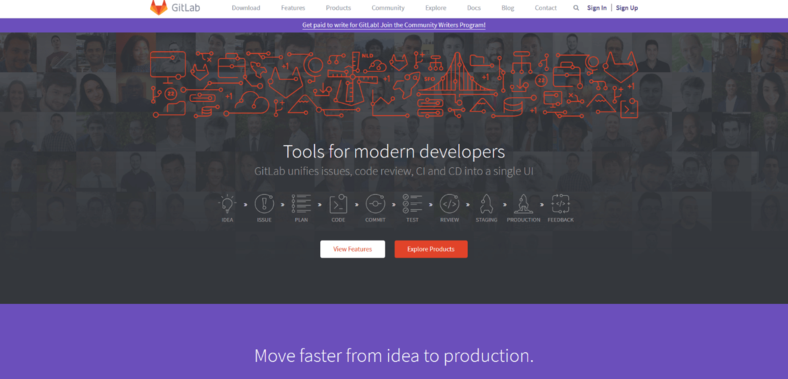
\includegraphics[width=15cm]{./Imagenes/git1} 
	\end{center}



	\item VSTS
	\\
	\\Visual Studio Team Services (VSTS) es un servicio alojado en la nube que se centra en equipos centrados en DevOps. Puede usar el repositorio integrado de Git si está buscando un repositorio privado. Pero en caso de que el proyecto ya esté alojado en GitHub o sea un proyecto de código abierto. VSTS puede actuar como un servidor de compilación que admite el repositorio alojado de terceros. La ruta para integrar GitHub es una de las mejores rutas predefinidas y, por lo tanto, es uno de esos servicios. Pero es eso lo que viene con un gran apoyo para la integración.
	
	\begin{center}
	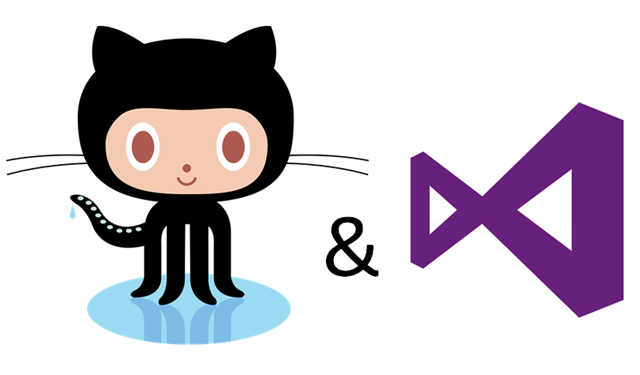
\includegraphics[width=10cm]{./Imagenes/git2} 
	\end{center}

	\item Bitbucket
	\\
	\\Bitbucket es un servicio de alojamiento basado en web, para los proyectos que utilizan el sistema de control de versiones Mercurial y Git. Bitbucket ofrece planes comerciales y gratuitos. Se ofrece cuentas gratuitas con un número ilimitado de repositorios privados .



	\begin{center}
	
\includegraphics[width=12cm]{./Imagenes/git3} 
	\end{center}


\item SourceForge
	\\
	\\A decir verdad, SourceForge ya estaba presente en el mercado antes de GitHub y de muchas otras alternativas open source y hubo una época en la que estaba considerada como la primera opción de código abierto. En 2015, la empresa tuvo algunos problemas con el malware, pero desde enero de 2016 va por el buen camino. Actualmente, SourceForge ofrece la autenticación multifactor, lo que armoniza con una orientación generalmente segura. Entre las características adicionales que pone a disposición de los usuarios se encuentran el sistema de seguimiento de incidentes y una lista de código incorporada.

	\begin{center}
	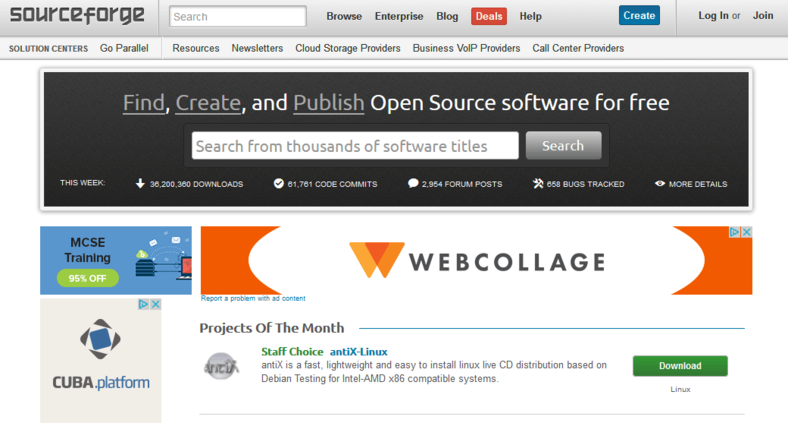
\includegraphics[width=15cm]{./Imagenes/git4} 
	\end{center}


	\item Cloud Source Repositories
	\\
	\\Tras el fracaso de Google Code, Cloud Source Repositories se encarga de la gestión de Google Cloud Platform. Con Cloud Source Repositories, que se encuentra en la versión beta, se pueden vincular otros repositorios vía GitHub o Bitbucket en función de las necesidades. En este caso, también es posible hacer uso de los repositorios propios de Google, los cuales se pueden guardar a través de la infraestructura de Google, lo que significa que tanto tu código como tus aplicaciones van de la mano.  La ventaja más importante de Cloud Source Repositories es que permite buscar código directamente a través del navegador.

	\begin{center}
	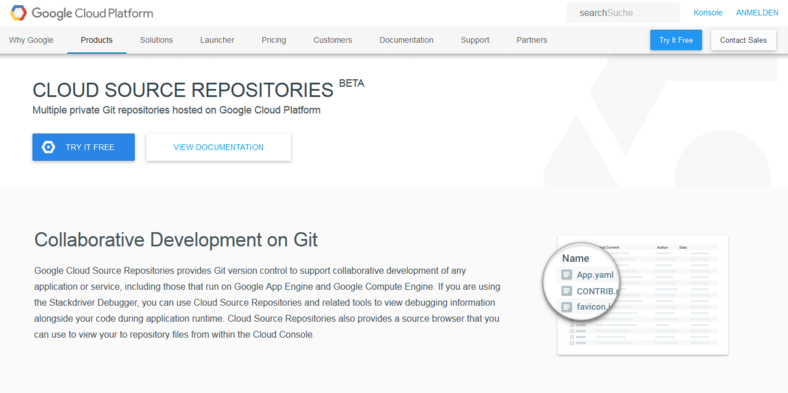
\includegraphics[width=10cm]{./Imagenes/git5} 
	\end{center}


	\item GitKraken
	\\
	\\GitKraken otorga un gran valor al ahorro de tiempo, algo que favorece a los usuarios a la hora de probar el código. Al sistema se le conoce, principalmente, por tener una interfaz muy vistosa, por centrarse en la velocidad y por el fácil manejo de Git. Con un práctico botón para deshacer operaciones se pueden revisar errores al momento, lo que hace más fácil el flujo de trabajo. La versión gratuita es apta para empresas con menos de 20 trabajadores o para organizaciones sin ánimo de lucro. La versión Pro, por su parte, ofrece características de gran utilidad, como por ejemplo el soporte de perfiles que permite separar proyectos con comodidad.



	\begin{center}
	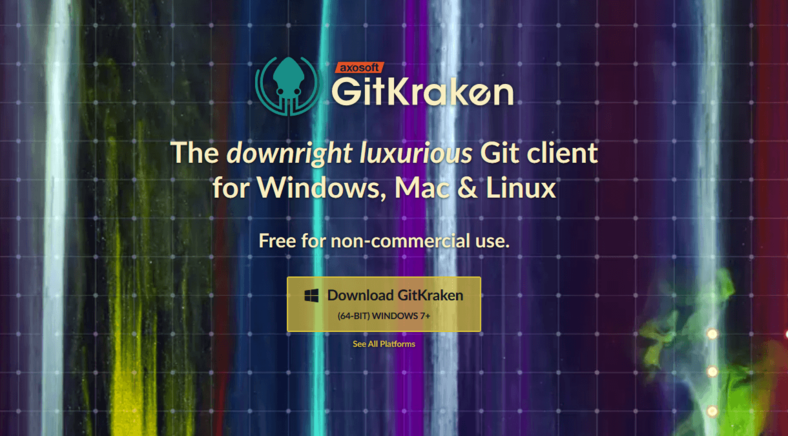
\includegraphics[width=10cm]{./Imagenes/git6} 
	\end{center}


\end{enumerate}
